\documentclass[../talk.tex]{subfiles}
\begin{document}

		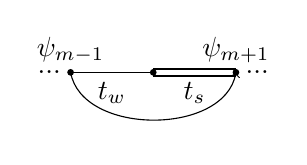
\begin{tikzpicture}[scale=.7]
    		\newcommand{\orig}{-1.5}
    		\newcommand{\trans}{1.5}
    		\newcommand{\vertspac}{-2.}
    		\newcommand{\rad}{2pt} % radii of the circles
    		
    		% set the style of the strong bonds
    		\tikzset{
    			strong/.style={
    				double,
    				double distance=\rad,
    				line width=0.5pt
    				}
    		}
    	
    		% bonds 
        	\draw[-] (\orig+\trans,0) -- (\orig+2*\trans,0) node [midway, below] {$t_{w}$};
			\draw[strong] (\orig+2*\trans,0) -- (\orig+3*\trans,0) node [midway, below] {$t_{s}$};	
    	
    		% sites
		    \filldraw (\orig+1*\trans,0) circle (0.05) node [left] {...} node [above] {$\psi_ {m-1}$};
		    \filldraw (\orig+2*\trans,0) circle (0.05) node [below] {};
		    \filldraw (\orig+3*\trans,0) circle (0.05) node [right] {...} node [above] {$\psi_{m+1}$};

			% arrow
			\path[->]
			(\orig+1*\trans,0) edge[bend right = 80] node [right] {} (\orig+3*\trans,0);
		      
		\end{tikzpicture}
		
\end{document}